\section{Toy Test Example, M-SDL}
\subsection*{General Setup}
Consider the linear multiple measurement vector model
\begin{align*}
\mathbf{Y} = \mathbf{AX},
\end{align*}
with $\mathbf{Y} \in \mathbb{R}^{m \times L}$ being a known measurement matrix, $\mathbf{A} \in \mathbb{R}^{m \times n}$ a known mixing matrix and $\mathbf{X} \in \mathbb{R}^{n \times L}$ being the source matrix we wish to recover in this case.
\\ \\
For this toy example consider a signal $\textbf{X}$ that is constructed as a merge of k independent signals. As such one column of X is one sample containing k active signals(sources) and n-k zero entries.\\
A random mixing matrix $\textbf{A}$ is generated as a random Normal distributed hence it has normalised columns:\\
\texttt{A = np.random.randn(m, n)  }  \\             
The measurements $\textbf{Y}$ is generated as the product of $\textbf{A}$ and $\textbf{X}$:\\
\texttt{Y = np.dot(A, X)}    \\ 
The error between all the elements of the true $\mathbf{X}$ and the recovered $\hat{\mathbf{X}}$ by using the mean square error (MSE):
\begin{align*}
\text{MSE} = \frac{1}{L} \sum_{i=1}^L (\mathbf{X} - \hat{\mathbf{X}}_i)^2
\end{align*}

Consider now $\textbf{Y}$ and $\textbf{A}$ known then by use of the M-SDL algorithm $\textbf{X}$ is sought recovered as $hat{\textbf{X}}$. The true $\textbf{X}$ is then to be used for comparison. 
\subsection*{Case 1 - $k>m$}
The following variables are used: 
\begin{itemize}
\item $m = 3$ (number of sensors)
\item $n = 8$ (number of sources)
\item $L = 100$ (number of samples)
\item No segmentations -- $\mathbf{Y} = \mathbf{AX}$
\item Iterations = 1000
\item $k = 4$ is active sources (row-wise) 
\end{itemize}


\subsection*{Results}
The MSE of case 1 was found to be $0.141$ when rounded to the nearest three decimal.
For visual comparison each active source are plotted against the reconstructed source in figure \ref{fig:case1_sources}. 
\begin{figure}[H]
\centering
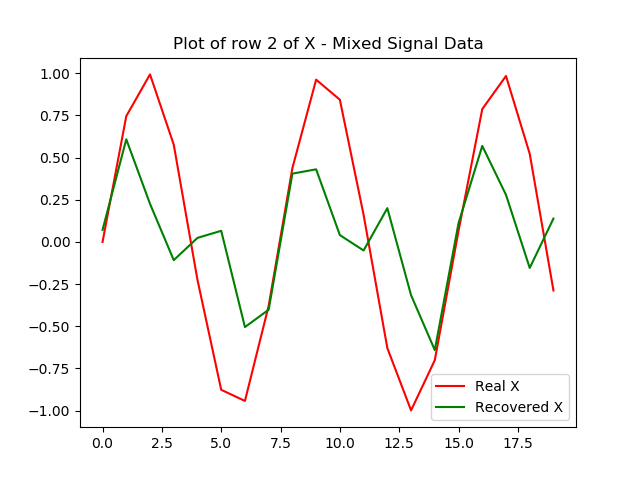
\includegraphics[width=\textwidth]{figures/cases/case1_1.png}
\caption{Comparison of each source for k = 4 }
\label{fig:case1_soures}
\end{figure}
\noindent
It is seen that one source was reconstructed as zero, that is the source was not reconstructed in the right location but in another. 
figure \ref{fig:case1_sample} show the comparison for one random chosen sample( row of X ),
\\ \\
For the next visualisation we look at the first 4 sources of $\mathbf{X}$ and $\hat{\mathbf{X}}$ to see how well the estimation is.
\begin{figure}[H]
\centering
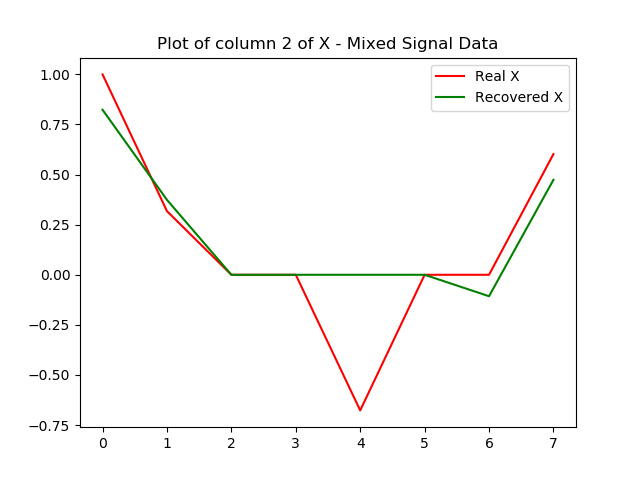
\includegraphics[width=\textwidth]{figures/cases/case1_2.png}
\caption{comparison of a single sample}
\label{fig:case1_sample}
\end{figure}
\noindent

\subsection*{Case 2 - $k<m$}
The following variables are used: 
\begin{itemize}
\item $m = 6$ (number of sensors)
\item $n = 8$ (number of sources)
\item $L = 100$ (number of samples)
\item No segmentations -- $\mathbf{Y} = \mathbf{AX}$
\item Iterations = 1000
\item $k = 4$ is active sources (row-wise) 
\end{itemize}

\subsection*{Results}
The MSE of case 1 was found to be $0.010$ when rounded to the nearest three decimal.
For visual comparison each active source are plotted against the reconstructed source in figure \ref{fig:case2_sources}. 
\begin{figure}[H]
\centering
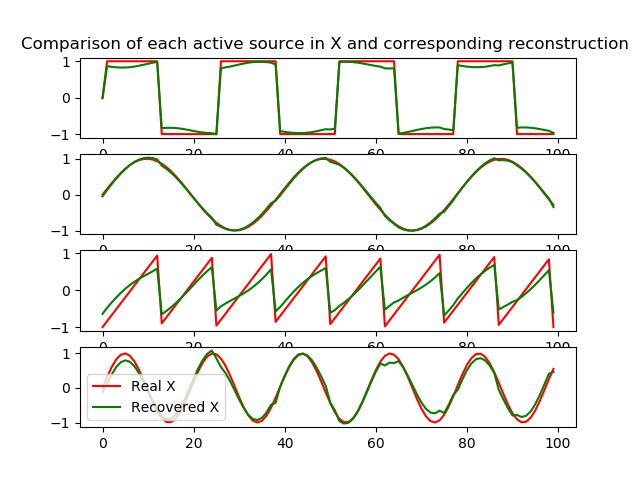
\includegraphics[width=\textwidth]{figures/cases/case2_1.png}
\caption{Comparison of each source for k = 4 }
\label{fig:case2_soures}
\end{figure}
\noindent
Figure \ref{fig:case2_sample} show the comparison for one random chosen sample( row of X ),
\\ \\
For the next visualisation we look at the first 4 sources of $\mathbf{X}$ and $\hat{\mathbf{X}}$ to see how well the estimation is.
\begin{figure}[H]
\centering
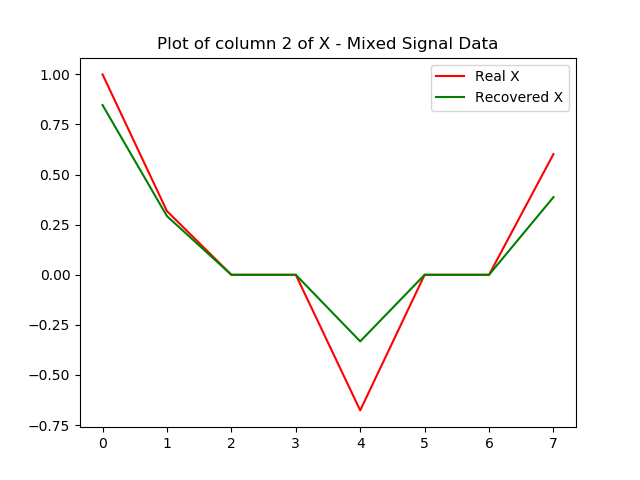
\includegraphics[width=\textwidth]{figures/cases/case2_2.png}
\caption{comparison of a single sample}
\label{fig:case2_sample}
\end{figure}
\noindent
